
%	\pagenumbering{gobble}
	
	\Large
	\begin{center}
		Resumé (Abstract)\\ 
		
		\hspace{10pt}
		
		% Author names and affiliations
		\large
		Martin DIGARD\\
		
		\hspace{10pt}
		
		\small
		martindigard@gmail.com\\
		
	\end{center}
	
	\hspace{10pt}
	
	\normalsize
	
	MÉMOIRE\\\\
	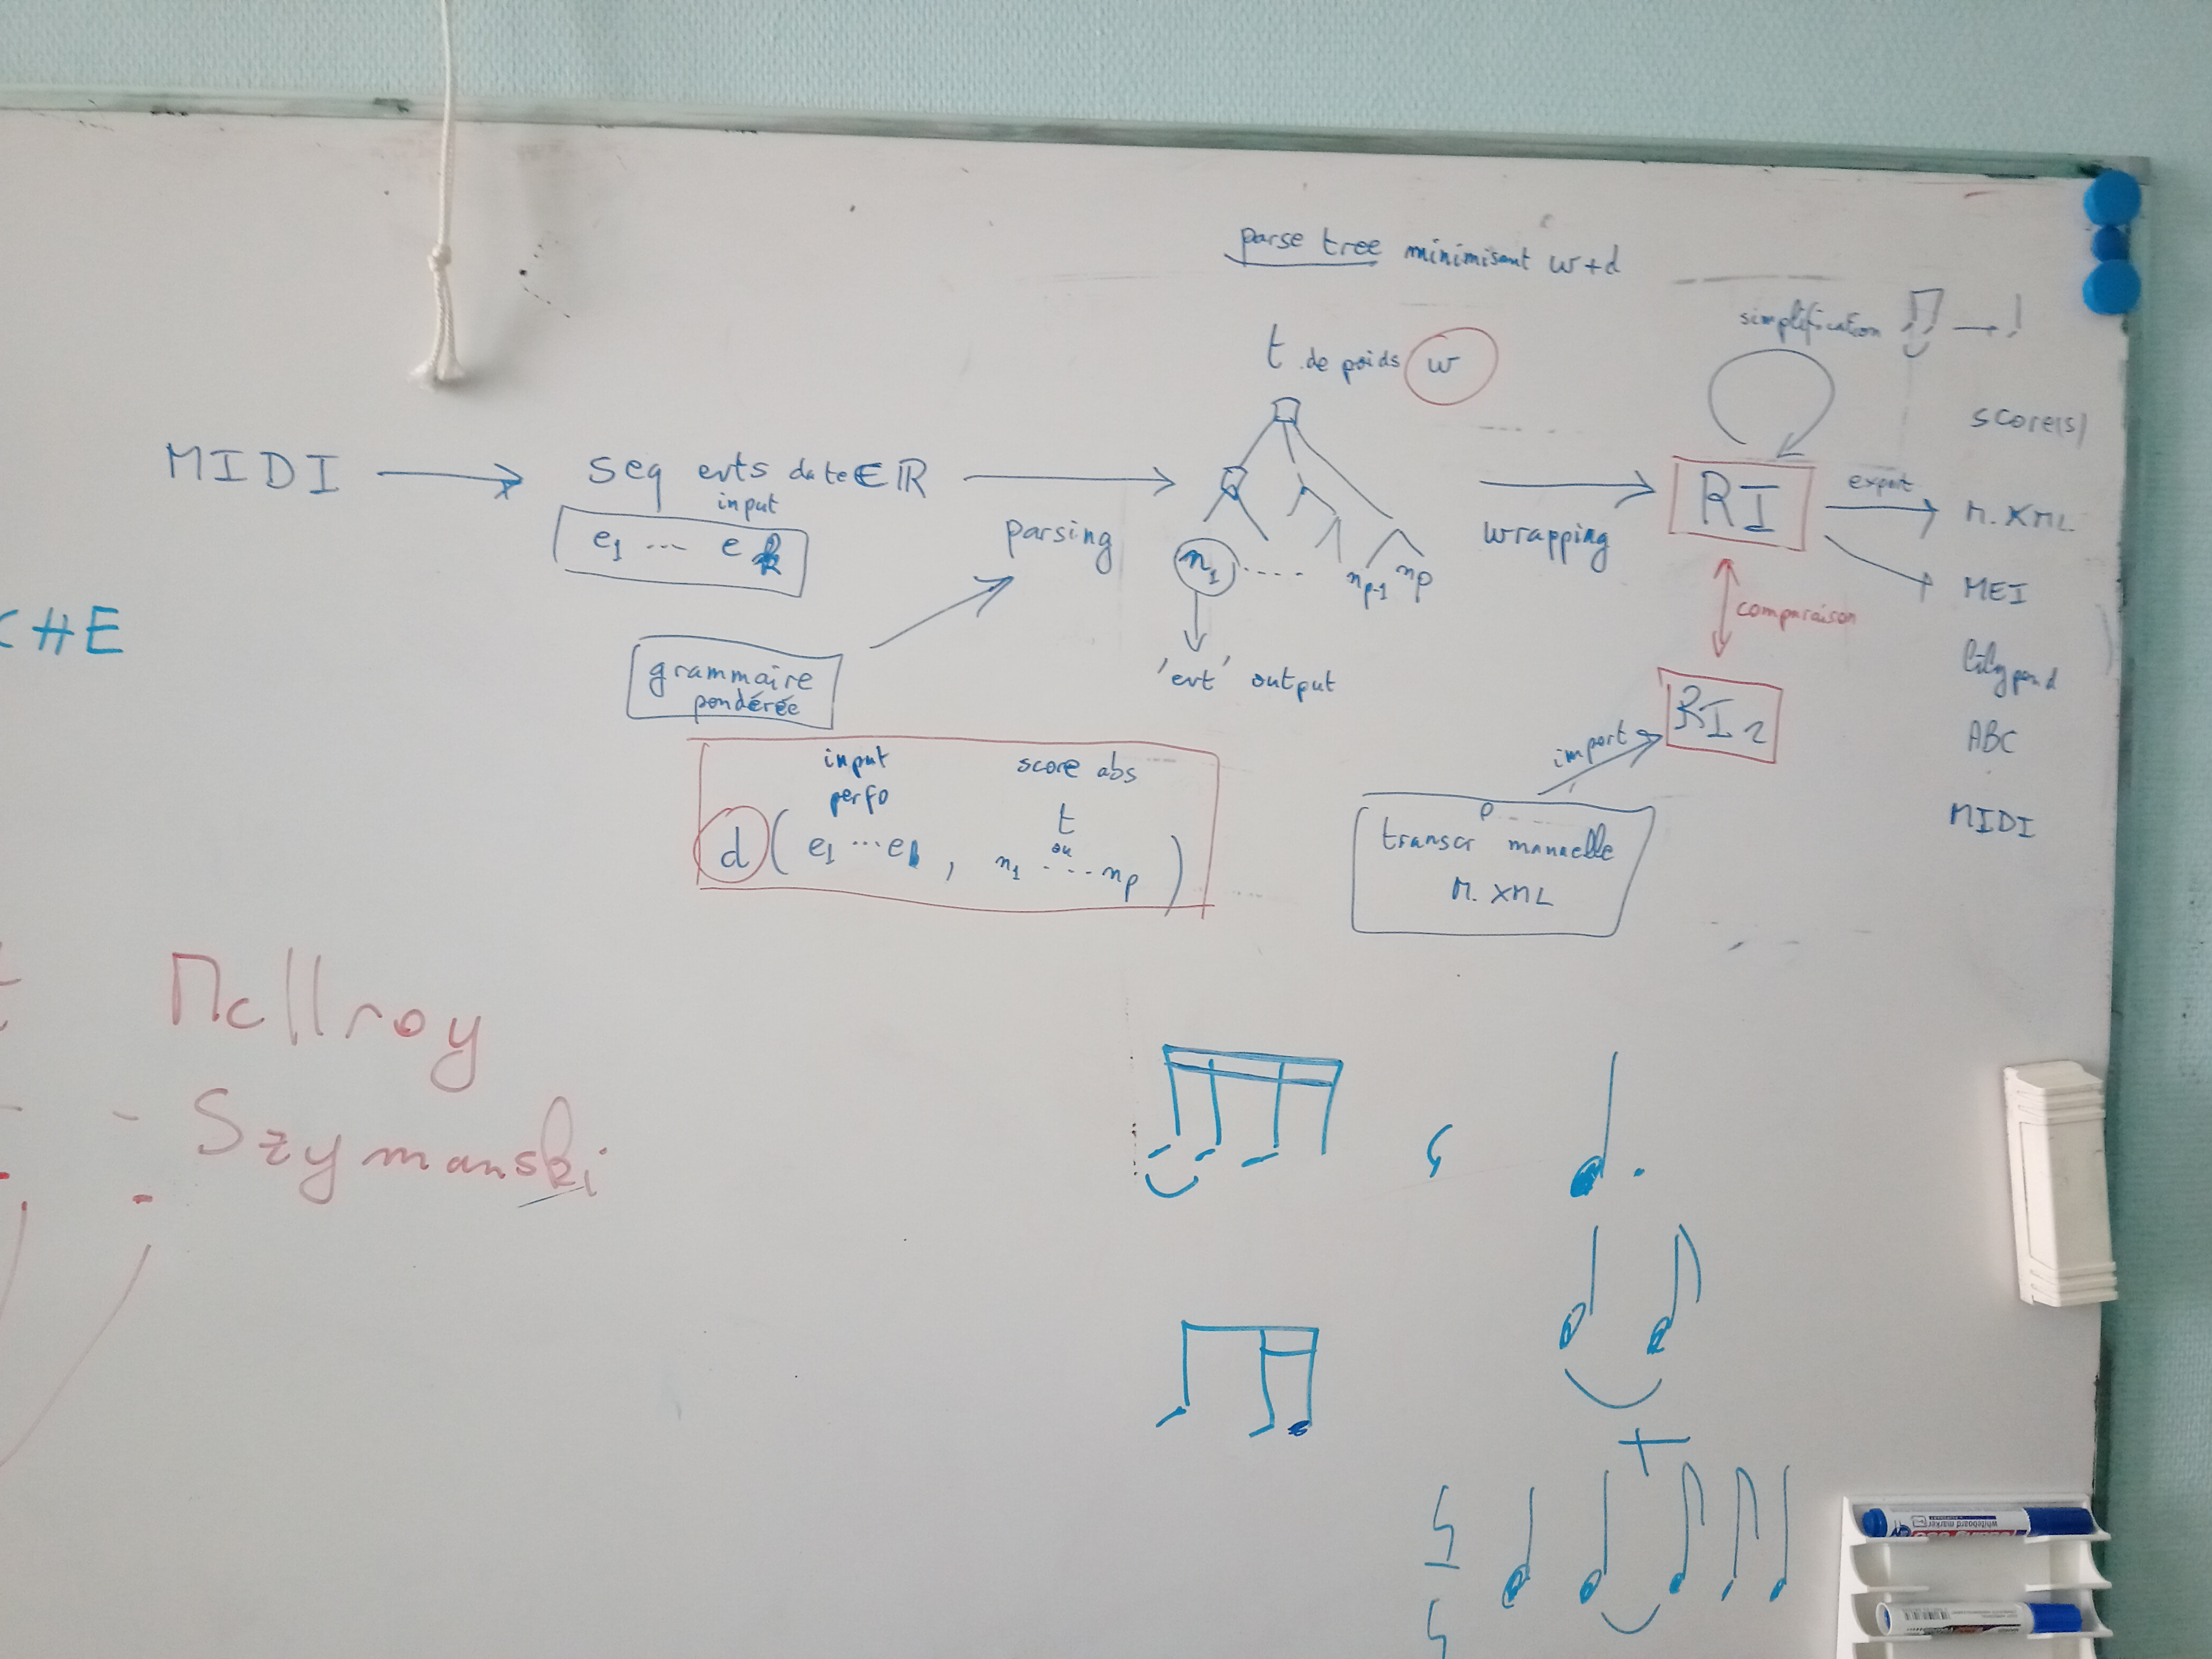
\includegraphics[height=80mm, width=80mm]{images/presentation/sujet_stage.jpg} \\\\
	En entrée : midi (séquence d’événements datés (piano roll) accompagné d’une grammaire pondérée)\\
	$\Rightarrow$ parsing\\
	$\Rightarrow$ global parsing tree\\
	$\Rightarrow$ RI (Représentation Intermédiaire) arbres locaux par intruments\\
	$\Rightarrow$ Sortie (xml, mei, lilypond,… )\\
	Minimiser la distance entre le midi et la représentation en arbre.\\\\
	Le but du stage est d’améliorer qparse, un outil de transcription et d’écriture automatique de la batterie (entre autre)\\\\
	\textbf{Le sujet de ce mémoire est de proposer une tâche de reconnaissance du regroupement des notes par les ligatures dans l’écriture de la batterie.}\\\\
	Pour cela, nous utiliserons la logique des systèmes (selon la définition agostinienne).\\$\Rightarrow$ Motif répétitif de plusieurs instruments coordonnées accompagnés d’un texte varié joué par un autre instrument de la batterie.\\\\Nous partirons de propositions génériques de systèmes (environs trois systèmes dans différents style de batterie) que nous tenterons de détecter dans le jeu de données groove.\\\\
	Nous travaillerons aussi sur la détection de répétitions sur plusieurs mesures afin de pouvoir corriger des erreurs sur une des mesures qui aurait dû être identique au autres mais qui présente des différences.
	
	
	